\documentclass[fontsize=8pt]{memoir} % use article if you want to use the old IPAD latex 
% otherwise use memoir class
\usepackage[utf8]{inputenc}
\usepackage[paperwidth=9cm, paperheight=11.5cm, top=0.5cm, left=0.5cm, right=0.5cm, bottom=0.5cm]{geometry}
\usepackage{graphicx}
\usepackage{url}
\usepackage{minted}
\usepackage{listings}
\usepackage{cite}
\renewcommand\bibname{References}


\newcommand{\Tool}{\textit{Ghost}\xspace}


% remove this if you wanted to use the old IPAD latex
% just added
\usepackage{tikz, blindtext}

\makechapterstyle{box}{
  \renewcommand*{\printchaptername}{}
  \renewcommand*{\chapnumfont}{\normalfont\sffamily\huge\bfseries}
  \renewcommand*{\printchapternum}{
    \flushright
    \begin{tikzpicture}
      \draw[fill,color=black] (0,0) rectangle (2cm,2cm);
      \draw[color=white] (1cm,1cm) node { \chapnumfont\thechapter };
    \end{tikzpicture}
  }
  \renewcommand*{\chaptitlefont}{\normalfont\sffamily\Huge\bfseries}
  \renewcommand*{\printchaptertitle}[1]{\flushright\chaptitlefont##1}
}

% end of just added


% fonts

%%\usepackage[scaled]{helvet}
%%\usepackage[defaultsans]{droidsans}
%%\usepackage[scaled]{libertine} 
%%\usepackage{lmodern} 

%% \usepackage[T1]{fontenc}
%% \usepackage{berasans}

% \usepackage[default]{gfsneohellenic}
% \usepackage[LGR,T1]{fontenc}

% \usepackage[light,math]{kurier}
% \usepackage[T1]{fontenc}

% \usepackage[math]{iwona}
% \usepackage[T1]{fontenc}

\usepackage{cmbright}
\usepackage[T1]{fontenc}

\renewcommand*\familydefault{\sfdefault}

% end of fonts

% uncomment this if you wanted to use the old IPAD latex
% \newcommand{\chapter}[2]{\begin{center}\section*{#1}\textbf{#2}\end{center}}

\usepackage{todo}
%Begin Decorative packages
\usepackage{type1cm}
\usepackage{lettrine}
\usepackage{fourier-orns}

\renewcommand{\pfbreakdisplay}{%
\decofourright\quad\decofourright\quad\decofourright
}

\usepackage{natbib}

%End decorative packages

\frenchspacing
\sloppy
\pagestyle{empty}

% remove this if you wanted to use the old IPAD latex
\chapterstyle{box}
\begin{document}

\title{Multistaging with Varying Preferences}
\author{by Huascar A. Sanchez}

\date{}
\maketitle
%\newpage
%\noindent
%[Disclaimer: For sake of convenience, I am temporarily using this latex template to improve the readability and accessibility of this document. Page margins and font size are increased, etc., giving the illusion of long sections. This template works perfectly in cases where you want to review this document from portable devices, such as the iPhone, iPad, Kindle, Android Tablet, etc.]
%% \newpage
\newpage
\begin{abstract}
This paper presents Program Design Mining, a data-driven approach 
for program design. This approach applies machine learning techniques,
such as structured prediction, nonparametric bayesian analysis, and 
program induction to facilitate new design interactions for program 
designers. Using ready available Web data, these techniques leverage 
the inherent structure of program designs to reason about and 
to manipulate the structural regularities of programs.
\end{abstract}

\chapter{Summary}{}
\label{sec:intro}

\section*{Overview} % (fold)
\label{sec:overview}

\startWith{w}{riting code} is not a manufacturing process, it's not 
always craftsmanship, it's design. Design is where developers add 
value faster than they add cost. However, design is both a complex 
and creative process, which can only be performed by developers after 
much practice (over many years). In today’s modern society, while the 
number of people with programming ability is growing at an astounding 
rate, the percentage of the population with a well-rounded program 
design experience remains in the single digits. This means that we are 
witnessing a growing gap between need and capacity. One can meet some of 
the need by using configurable programs with canned behavior, but these 
restrict both creativity and problem solving (i.e., capacity) to those 
anticipated by the creators of those programs. Therefore, it is critical 
that we find programmatic ways in which we can help both traditionally 
and non-traditionally educated programmers borrow the same skills and 
creativity of the formally trained pros and still express themselves.

In a new research direction, we term Program Design Mining, we propose  
making some of the abilities, which allow star developers to succeed, 
available to citizen programmers by applying machine learning to program 
design. We will leverage existing design knowledge on the Web (e.g., 
GitHub software repositories) to help program designers. On the Web, 
every well-written program represents a concrete example of human 
creativity and design wisdom. Given these ready available Web data, 
Program Design Mining will identify and then manipulate structural 
regularities \cite{minsky1991law} of (object-oriented) programs, such idioms, 
coding rules, and design patterns. Program Design Mining exploits three machine 
learning applications to enable new interaction mechanisms for program 
design: (1) structured prediction \cite{collins2002discriminative} for 
finding static and semantic correspondences between programs, which can 
be used by programmers to transfer the structural regularities from one 
program into the structure of the other; (2) program induction \cite{lake2015human} 
for learning generative models that could help program designers manipulate 
(and evolve) the transfered structural regularities; and (3) nonparametric 
bayesian analysis \cite{allamanis2014mining} for dealing with incompatibilities 
between structural regularities.

All of these techniques leverage the inherent structure of program designs. 
Well-written (object-oriented) programs, for example, exhibit many structural 
regularities\footnote{These regularities explicitly mold programs with design 
and coding principles that intend to improve their quality} and their 
identification and manipulation improves with experience. Machine learning 
can eliminate the need for gaining design experience, as it allows us to learn 
from existing design knowledge. On the Web data, every Java class is associated 
with an abstract syntax tree. This information can be used along with the change 
history of this class to reason about and manipulate such structural regularities, 
closer to way experienced developers will do. 

With Program Design Mining, we will decouple the ability of designing quality 
programs from the time it takes to fine tune such an ability. Design wisdom 
will not come with many years of practice \cite{weiser1983programming, 
winslow1996programming}. It will come with less time and through new design 
workflows (e.g., code transformations) learned from programs' change 
history. Developers will be able to evolve their programs with sound design and 
coding principles. At every opportunity, developers will try different a design 
alternative and experience the results. If they like, then they will keep it, 
otherwise, they discard it. Program design mining will exploit ready available 
Web data to foster design inspiration when innovation is required, and thus 
reducing the gap between need and capacity.

In what follows, we will cover the intellectual merit of data-driven 
approaches for program design, as well as the broader impact of Program 
Design Mining.

\section*{Intellectual Merit} % (fold)
\label{sec:merit}

This project proposes a novel approach for program design and 
evolution. Encouraged by many recent advances in code transplantation, 
data-driven Web design, and software evolution simulation, we 
present Program Design Mining. The key innovations behind this 
approach include:

\begin{enumerate}
	\item Data-driven program design. Establish new design workflows 
	from existing design knowledge. These workflows allow citizen 
	programmers to automatically transfer the structural regularities 
	from a well-written program into the style and structure of another.  
	\item Semi-automatic program design tuning. Generate structural 
	regularities recommendations by analyzing learned regularities online; 
	i.e., in parallel with structured prediction, which allows the 
	recommendations to adapt to transfer incompatibilities. Programmers 
	can provide feedback on the recommendations, which is taken into 
	account for subsequent recommendations.	
	\item Operationalization and evolution of learned regularities. 
	On the to-be-collected Web data, for example, every Java class is associated 
	with an abstract syntax tree. Along with its change history, we can use 
	this abstract representation to reason about and manipulate programs 
	with \textit{similar} structures.
\end{enumerate}

\section*{Broader Impact} % (fold)
\label{sec:impact}

Computer systems affect most parts of our lives. Countless examples of 
the grave consequences caused by poorly crafted software systems include 
severe financial damages or even the loss of lives. With the looming 
advent of Citizen Programming, the amount of code to be produced by 
opportunistic programmers grows at a staggering pace, demanding for more 
automated tools to ensure software quality. This project contributes a 
data-driven program construction technique that will help people with 
programming ability to write code closer to what an experienced programmer 
would write. Further, the project will create a suite of benchmarks to 
serve as baseline for other automated program construction tools.

SRI International make considerable contributions to education, research, 
and technology transfer to industry through its freely distributed tools 
and academic visitor programs such as include summer internships for graduate 
students that encourage applications from minority students.
\chapter{Project Description}{}
\label{sec:related}

\startWith{d}{evelopers} frequently rely on templates (e.g., 
recipes in Eclipse) when designing programs in modern Integrated 
Development Environments (IDEs). While these templates provide 
a simple mechanism for implementing canned behavior, there are a 
few issues that hinder their applicability: (1) Templates creation 
is tedious, which restricts productivity, and (2) Templates rigidity 
limits customization and creativity.

Program Design Mining will implement a data-driven approach for 
program design. This approach consists of a platform, and a set of 
algorithms, such as: 

\begin{enumerate}
	\item A new structured prediction algorithm for rapidly transferring 
	the structural regularities of well-written (object-oriented) programs 
	into the style and structure of another one.
	\item A new program induction algorithm for learning and operationalizing 
	(composition or remix) learned templates to foster program design 
	inspiration when innovation is required.
	\item A new semi-automatic (human-in-the-loop) program evolution algorithm 
	for bouncing program design alternatives (and evolving programs). 
\end{enumerate}

State of the art data-driven tools for program synthesis, program 
repair, and code transplantation, such as X, Y, and Z, focus 
on the code itself and struggle with transferring code from one system 
to another, because of the nontrivial modifications needed to relocate 
unrelated foreign code fragments into new programs. 
\chapter{Fundamentals}{}
\label{sec:fundamentals}

% \fancybreak{\pfbreakdisplay}

\lettrine[lraise=0.1, nindent=0em, slope=-.5em]{T} {HIS CHAPTER} sets the stage for the complete description of \Tool in the next chapters.

\fancybreak{\pfbreakdisplay}

\section{Eager vs. Lazy Evolution}
\label{sec:eagervslazy}

\uppercase{\Tool} builds on an eager program evolution policy, a policy that is executed with minimal control from developers. Below, this policy and its opposite---a lazy program evolution policy, a policy that is executed with moderate control from developers---are described.

\subsection{Eager Evolution}

Eager evolution is the policy of continually making code changes to one or more search results, and feeding any suitability scrutiny on the outcome back into the search process\footnote{A rapid experimentation of example code}. A process that has such a policy operates under two assumptions:

\begin{enumerate}
	\item Code retargeting is a \emph{cheap}---efficient---operation, and
	\item Code retargeting ought to be done often
\end{enumerate}

Code retargeting ought to be done often in dynamic and exploratory scenarios---i.e., when the developer is working in an unfamiliar domain~\cite{Brandt:2009ew}. In such a scenario the type and number of code examples may quickly change as further searches are performed. Therefore, it makes sense to frequently retarget any results to get a better picture of the results and their suitability~\cite{Fowler:1999vp, Brandt:2009ew}. 

This policy accounts for the fact that it may not be possible to completely and safely perform code retargeting on certain snippets. In this case, the retargeting operation will result in an error. Therefore, it can hypothesized that if changes such as renaming functions or parameters, adding or removing arguments, or reorganizing structures cannot be applied, then the cognitive distance of the snippet's abstractions is high and the pay-off for reusing it is relatively small. Consequently, this found result may not be worth the developer's effort and thus it can be discarded.    

The expected advantages of eager retargeting are:

\begin{enumerate}
	\item The example code is more likely to match what the end user had in mind.
	\item The end users can have more confidence sooner that the picked examples were the right ones.
	\item The end users can waste less time agonizing over modification problems they find costly to fix. 
\end{enumerate}

% 
% \fancybreak{\pfbreakdisplay}

\subsection{Lazy Evolution}

Lazy evolution is the policy of only making code changes to a result at the point of integration in the IDE. Under this policy, there is no guarantee---beyond relative ranking values---of the result's suitability. Due to this uncertainty, a process that has such a policy operates under two assumptions:

\begin{enumerate}
	\item Code retargeting is an \emph{expensive} operation, and
	\item Code retargeting ought to be done only at the point of integration
\end{enumerate}

A process that has such a policy assumes code retargeting is a costly operation~\cite{Brandt:2009ew, Wightman:2012gc}. This is based on the observation that developers, under this policy, cannot plan the impact of choosing a code example on their current work until they have tried it. This means that---at the point of integration---unrelated and/or unsuitable results are more likely to require many more code changes than suitable results.
% 
% \fancybreak{\pfbreakdisplay}

\subsection{Reasoning about these two policies}

Intuitively, one needs to figure out whether an eager code retargeting policy leads to a \emph{cheaper} and thus \emph{faster} code search process than its opposite. 

One could model the notion of ``cost'' to retarget code examples with the following components:

\begin{enumerate}
	\item Code understanding
	\item Code modification
	\item Code disturbance
\end{enumerate}
 
The code understanding effort takes into account the time needed to carry out program comprehension actions, such as locating the snippet, doing content analysis, screening snippets, etc. This effort is denoted by $U_{s}$, which is defined as the average effort required before starting the actual retargeting actions.

Code modification efforts represents the cost of changing the necessary tokens in a snippet. For a sequence of tokens `a', let $\alpha^{+}(a)$ denote the cost of adding changes to `a'. This term is formulated as: 

\begin{equation}
	\alpha(S_{i}) = C_{s} \times (\sum_{a \in S_{i}}\alpha^{+}(a))
	\label{costmodification}
\end{equation} where $C_{s}$ is the average estimated time for one generic snippet change to be performed by the developer.

Code disturbance expresses the cost of tinkering~\cite{Jadud:2006ir} when facing an unexpected situation. It is assumed that code disturbance is proportional to the amount of interruptions---e.g., unpredictable errors---experienced by a developer during retargeting and how long each interruption takes as a snippet varies. This term is formulated as:

\begin{equation}
	\delta(S_{i}) = T_{s} \times Interruption(S_i)
	\label{costmodification}
\end{equation} where $T_{s}$ is the average estimated time an interruption takes, $S_i$ the snippet being modified, and $Interruption(S_i)$ the number of interruptions experienced when changing a snippet $S_i$. 

Therefore, the overall retargeting cost is defined as:

\begin{equation}
	cost(S_1, ..., S_n) = U_s + (\sum_{i=1}^{n}(\alpha(S_{i}) + \delta(S_{i})))
	\label{totalWork}
\end{equation} where $S_1, ..., S_n$ are different snippet variations that can be derived from retargeting actions.

From the above model, one can assume that the \emph{winner} policy is the one with the smallest total cost.

Eager retargeting assumes a low cost. This is based on the observation that unsuitable results---i.e., results that cannot be retargeted---are excluded more often, leaving the developer only suitable choices to handle. Not only does the time to find suitable choices improves, but also less time (a.k.a., wasted) agonizing over modification problems that are costly to fix. Obviously, this leads to a low total cost. 

In contrast, as it has been already suggested in previous work~\cite{Brandt:2009ew, Wightman:2012gc}, a lazy retargeting policy assumes a high cost. Under this policy, it is common for one to look at each promising result (suitable or unsuitable) in its entirety\footnote{all the way to try to retarget each individual result at the IDE.}---usually one by one. The problem with this is that the feedback, revealing the suitability of an example, may take a significant time to get back to the developer. By then so many changes have been made that there is often no clear ending for the task (more disturbance). The developer's only recourse is to restart the search process. Not only does this lead to a high total cost, but also to a sluggish searching interaction~\cite{Gray:2000im}.  

Since the major ``cost'' of each policy is directly connected to the time spent by the developer searching for suitable code, a policy leading to a \emph{cheaper} code search process leads also to a \emph{faster} code search process.

% 
% \section{What rules should guide the Retargeting of found code?}
% \label{sec:sniprrules}
% 
% \uppercase{\Tool} models code searching as a short cycle of alternating query, screen, and retarget phases: found code is retargeted with commands issued just following to the displaying of a result set or prior to issuing a query (Figure). This model is operationalized using a state machine (Figure): during browsing, reported results are added to a queue; when the user .    
% 
% when the user edits code, all pages in the queue are assigned to new characters. 
\fancybreak{\pfbreakdisplay}

\section{How to start developing with \uppercase{\Tool}}
\label{sec:sniprscenario}

A scenario will be given to help introduce the main interaction techniques. \uppercase{\Tool} offers two choices for interacting with code-centric sites: to issue queries and retargeting operations separately, or to intermix queries and retargeting operations. For sake of clarity, this section will focus on the former.

Olivia is an amateur developer and open source evangelist who frequently practices search-driven development at her workplace. Olivia would like to transition a sentiment analysis tool (that uses the Twitter API) to use the Facebook API. The updated tool should handle the sentiment classification of status updates in Facebook. She wants status updates to be classified dynamically. She is familiar with Java and has some Machine Learning experience, but does not consider herself an expert developer.

Olivia starts by opening Twist---a \uppercase{\Tool}-aware snippet-centric search engine she frequently visits for discovering open source libraries. This engine spans large sets of open source projects; mostly indexed from a variety of project hosting sites, such as Github, and Google code. Olivia interacts with Twist by using Twist's REPL\footnote{\url{http://en.wikipedia.org/wiki/Read-eval-print_loop}}. Twist allows Olivia to use queries and/or code retargeting operations to do code searching. The design of Twist will be described in Chapter~\ref{chap:twist}. Figure~\ref{fig:twist} shows Twist's Web interface. 

% \begin{figure}[!ht]
%     \centering
%     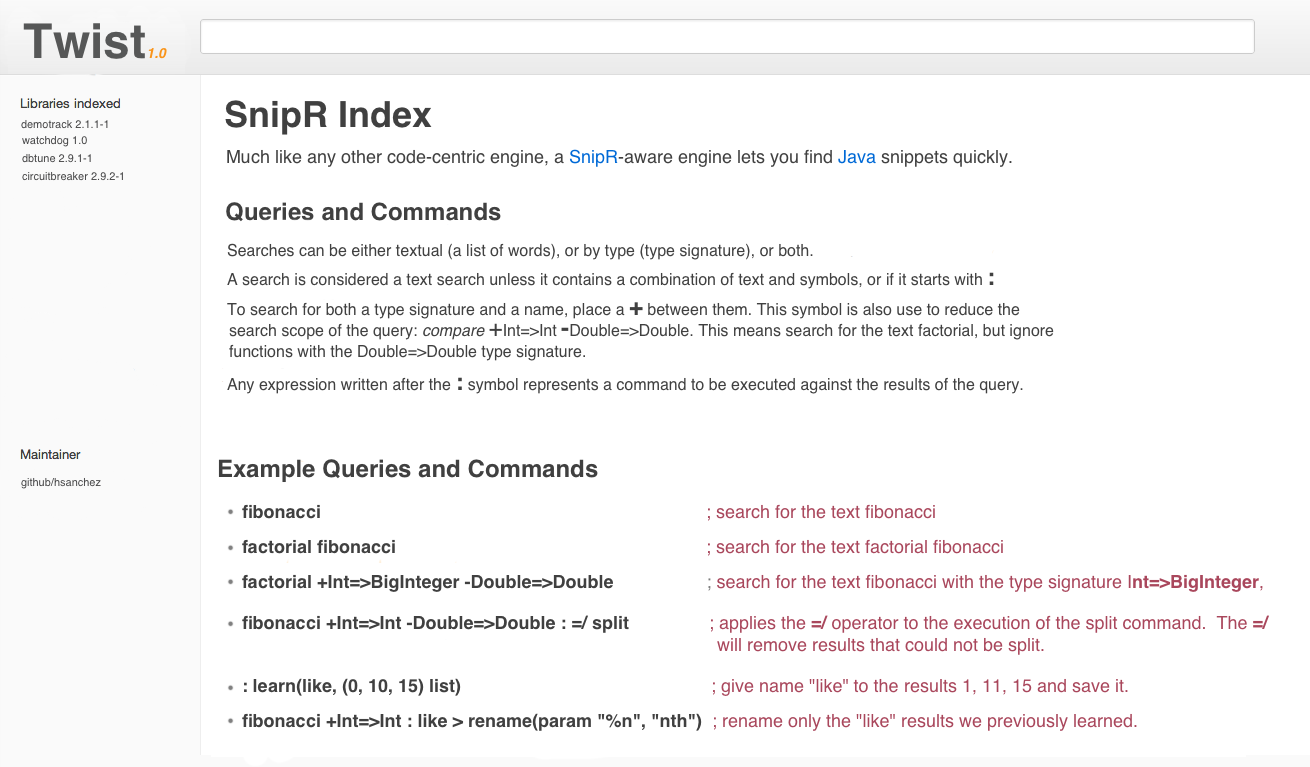
\includegraphics[width=\textwidth]{images/twistsite}
%     \caption{Twist's Web Interface.}
%     \label{fig:twist}
% \end{figure}
% \pagebreak

To start searching for code examples, Olivia issues a query targeting Facebook APIs written in Java. Olivia specifically looks for functionality that deals with status or post updates. For some unexplained reason, she does not want any Android\footnote{\url{http://www.android.com}} specific source code. Consequently, Olivia's first query contains a list of words matching her intent and a reduction in search scope. Figure~\ref{fig:twistquery} shows this query and the results produced by it. 

% \begin{figure}[!ht]
%     \centering
%     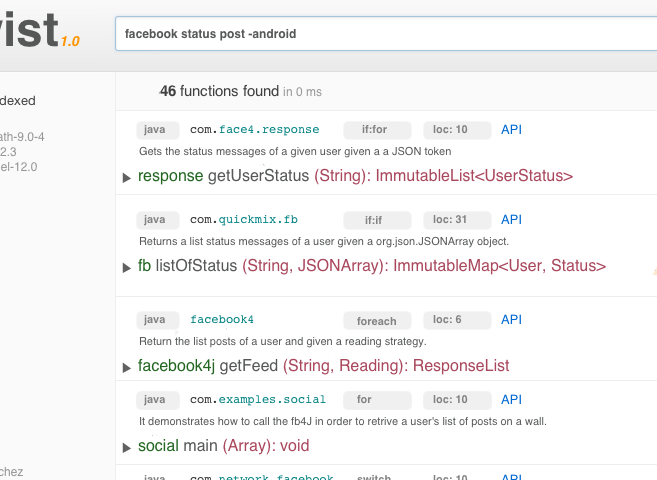
\includegraphics[width=\textwidth]{images/twistquery}
%     \caption{Olvia's first query, which targets Facebook APIs written in Java.}
%     \label{fig:twistquery}
% \end{figure}
% \pagebreak

Olivia tries to screen all of the results but gives up after some time. There is a lot of good stuff, but she does not have the time to look at every single result. Consequently, she uses Twist's functionality to her own advantage. She issues a command that rejects results exceeding 20 lines of code (Figure~\ref{fig:twistslash}), resulting in a more manageable set of 16 results. Consequently, Olivia's screening efforts will be reduced.

% \begin{figure}[!ht]
%     \centering
%     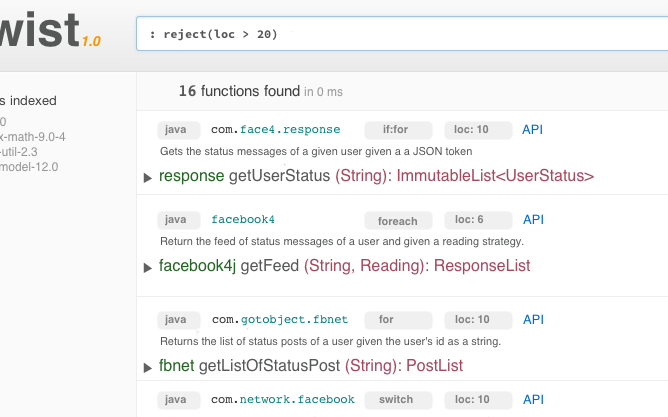
\includegraphics[width=\textwidth]{images/twistslash}
%     \caption{Olivia rejects the code examples whose size exceeds 20 lines of code. The
% 	 reject operation takes as an input the list of current results and an anonymous function,
% 	 which is applied to every result in that list.}
%     \label{fig:twistslash}
% \end{figure}  

Some of these results (Figure~\ref{fig:twistslash}) have highly coupled dependencies that Olivia is not interested in using, such as the ImmutableList dependency from the Google's Guava library\footnote{\url{http://code.google.com/p/guava-libraries/}}. She then issues a retargeting request that replaces those dependencies with APIs found in the Java SDK. Olivia can specify these dependencies by typing an associated abbreviation; e.g., ImmutableList can be written as IL or ImL. The execution of this request reloads the Twist page, listing the successfully retargeted snippets and adding red markers next to the failed-to-retarget snippets (Figure~\ref{fig:twistretarget}). These markers indicate Olivia should not spend any further effort on these results. 

% \begin{figure}[!ht]
%     \centering
%     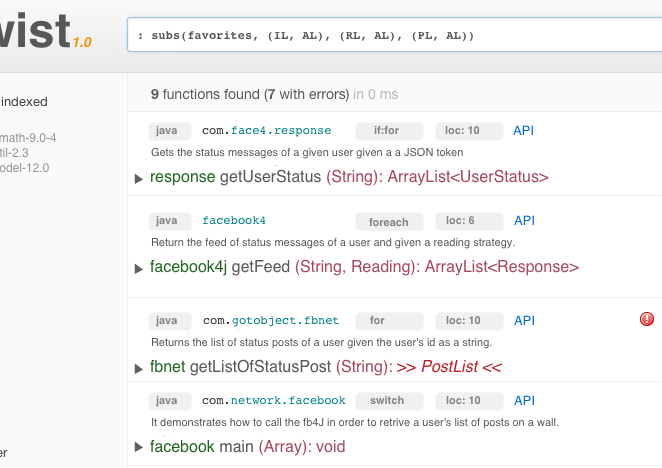
\includegraphics[width=\textwidth]{images/twistretarget}
%     \caption{Olivia issues the subs command against the favorites sub list. This command
% 	 replaces one type for another. Favorites is a sub list extracted from the main list of results and its defined as: learn(favorites, ((0 list), (1 list), ...).}
%     \label{fig:twistretarget}
% \end{figure}

For Olivia, the whole idea of having the failed-to-retarget snippets around is distracting. Therefore, she issues another command which drops any failed-to-retarget results from the current list of results. Figure~\ref{fig:twistclean} shows this action. 

% \begin{figure}[!ht]
%     \centering
%     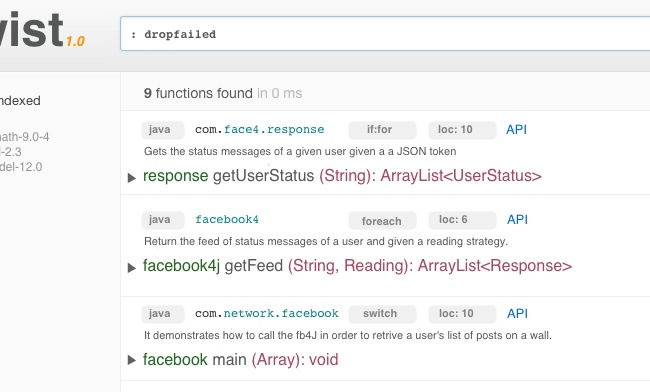
\includegraphics[width=\textwidth]{images/twistclean}
%     \caption{Olivia issues a user-defined command, named dropfailed, which will drop
% 	 any failed-to-retarget results from the current list. The dropfailed was defined as :
% 	 learn(dropfailed, reject(list, err == false))}
%     \label{fig:twistclean}
% \end{figure} 

At this point, Olivia could actually issue more commands. However, she decides to arbitrarily click on individual results that she sees as good candidates for additional retargeting. This action offers the choice for further retargeting to gain more confidence of these results' suitability (see Figure~\ref{fig:basealternative} for an example). She then invokes a few additional commands: rename functions, and change a condition-controlled loop (e.g., for loop) to another one (e.g., while loop), matching what Olivia had in mind for how and what status updates are obtained\footnote{This process can continue (See Eager retargeting policy in Section~\ref{sec:eagervslazy}) until Olivia decides to stop.}. Again, any unsuitable results are filtered out and thus the number of results to be inspected by Olivia is reduced.

Continuing her information gathering, Olivia may continue retargeting results until there are no more results to screen or to not like any of the different variations. This can happen, which can lead Olivia to modify her previous queries to obtain similar or different results than she had previously obtained.

When she is satisfied with the resulting code examples, she can evaluate these results in more detail and thus pick the most suitable example she can integrate into her own code.


\chapter{Algorithms}{}
\label{sec:algos}

\lettrine[lraise=0.1, nindent=0em, slope=-.5em]{T} {HIS CHAPTER} sets
\chapter{Evaluation}{}
\label{sec:eval}

\lettrine[lraise=0.1, nindent=0em, slope=-.5em]{T} {HIS CHAPTER} sets
\chapter{Conclusion}{}
\label{sec:conclusion}

\lettrine[lraise=0.1, nindent=0em, slope=-.5em]{T}{HIS DOCUMENT HAS} introduced

\todos
\bibliographystyle{abbrv}
\bibliography{main}

\end{document}